\chapter{Introduction}
\label{intro}

\section{Background}

Offshore monopiles are increasingly preferred for wind farm installations, owing to their benefits in clean energy generation and convenient deployment. These cylindrical steel structures are driven into the seabed to establish a stable foundation for wind turbines. While offshore wind energy holds promise as a source of clean and sustainable power, the adoption of offshore monopiles introduces specific engineering challenges. A primary concern associated with offshore monopiles is addressing potential issues related to excessive pile displacements induced during both their installation and operation phases \citep{byrne2003,randolph2005}. Excessive movements in the piles can result in significant displacements and rotations within supporting structures, subsequently leading to damage or structural instability. Consequently, accurate prediction and effective management of pile deformations become paramount when designing and analyzing support systems for offshore monopile installations.





After soil properties, design loads and pile dimensions are acquired from a technical report, estimating the pile response is typically done through empirical solutions in guidelines or numerical simulations. Several design methods have been provided in the design codes \citep{api2011,bhattacharya2019} to predict offshore pile $p-y$ curve. However, it is challenging to incorporate all influential factors, such as pile length, soil layer, soil properties and loading conditions into a simplified empirical model. Rapid advancement of computational techniques has facilitated the numerical models \citep{randolph2017,taborda2020,zdravkovic2020,royston2022}, serving as a potent analytical tool. Nonetheless, it necessitates a substantial number of simulation runs. This presents a significant challenge on the back-calculation of parameter properties, especially in the context of inverse and predictive analysis.

In recent research endeavors, Bayesian probability frameworks have garnered increasing recognition as an efficacious approach for inverse parameter estimation and response prediction \citep{finno2005,nakamura2011,hsein2013,nguyen2016,wagner2020,jin2021,tao2021,buckley2023,tang2023}. In such circumstances, the Bayesian framework emerges as a powerful tool within the probabilistic context, facilitating parameter learning and informed decision-making. However, in high dimensions (typically in geotechnical areas), the computational cost of such model is high. Traditional Monte Carlo methods for UQ or manually overcoming this limitation is nearly impossible. There is an urgent requirement to tackle these issues. Luckily, the components necessary to address such problems have been already at our disposal. The UQ and machine learning communities have developed methodologies to efficiently address large-scale data models and disseminate uncertainties. However, in geotechnical engineering, there is a noticeable absense of guidlines for UQ area. Based on this, a data-driven dynamic UQ framework is hoped to be constructed and enable the real time information sharing between the models and measurements. 

In practice, through adaptive Bayesian updating on the identified parameters and reduce the uncertainties on offshore piles, a field engineer would benefit from: (1) properly accounting the uncertainties of input variables; (2) real-time monitoring and adaptively predicting the pile response in probabilistic setting; (3) providing an efficient tool for data-driven decision making on pile operation and design. In the context of offshore engineering, in particular, it will show substantial potentials in various domains, including health monitoring, pile penetration and long-term bearing capacities \citep{wang2021,zhao2023,stuyts2023}. 



\section{Problem statement}

Modern pile installation and proper estimation is becoming increasingly complex and vital to the reliability and permanence of the foundation in question. However, in the construction process, uncertainties and insufficient information (e.g., soil parameters) lead to inaccurate predictions of pile responses. The source of uncertainties may come from various reasons. Dealing with different uncertainties sources is a challenging task. One typical uncertainty source can be illustrated in \cref{fig: Cowden_cpt}, which shows uncertainties sources:

% \setlength{\parskip}{0pt}
% \setlist[itemize]{itemsep=0pt,topsep=0pt,parsep=0pt,partopsep=0pt}

\begin{itemize}[left=0pt]

    \item Fluctuating curve indicates the spatial variability
    \item Non-uniformity exists between in-situ test and laboratory experiment

\end{itemize}
\vspace{0.2cm}

Furthermore, geotechnical engineering problems inherently belong to the high-dimensional realm with substantial uncertainties. The substantial quantity of unknown distribution parameters might be too extensive for precise inference, given the small size of the accessible data, resulting in an underdetermined problem. Although some well-established approaches for fitting pile deformations are proposed to infer the underlying soil parameters and reduce the uncertainties, addressing this challenge becomes intricate when confronted with a multitude of input variables (i.e., $\mathcal{O}(10^2-10^4)$) \citep{lataniotis2019}. 
Even if an adequate probabilistic input model can be obtained, performing the inference analysis through Monte Carlo simulation is still expensive. This poses challenges in understanding uncertainties and providing timely predictions for pile design. In these scenarios, it becomes practical to replace the computational model with a surrogate. Nevertheless, as dimensions increase, the efficacy of surrogate models diminishes, accompanied by escalating computational and storage expenses. This quandary is widely acknowledged as the \textit{curse of dimensionality} \citep{verleysen2005}. Computing the surrogate may become challenging, especially when confronted with a substantial number of input parameters \citep{lataniotis2019}.


\begin{figure}[htbp]
    \center
    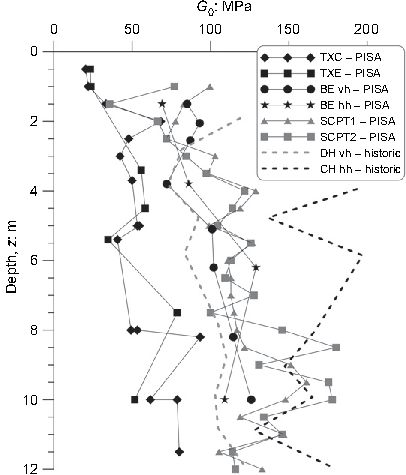
\includegraphics[width = 90mm]{Figures/figure-Cowden.pdf}
    \caption{Stiffness characteristics at Cowden from \protect\cite{zdravkovic2020}}
    \label{fig: Cowden_cpt}
\end{figure}






\section{Objectives and outlines}
\subsubsection{Objectives:}
This thesis aims to construct a resilient and scalable framework for uncertainty quantification, extending its applicability beyond offshore piles. This endeavor will leverage cutting-edge methodologies in surrogate modeling, uncertainty quantification, probabilistic graphical model and control theory, all geared towards facilitating extensive predictive digital twin capabilities. In particular, the specific goals of this thesis are:
\begin{itemize}[left=0pt]
    \item Develop a surrogate model suitable, not limited for offshore piles, for structures characterized by high input dimensions.
    
    \item Accelerate Bayesian inversion calculations for identified parameters to reduce the uncertainties, and providing real-time pile response predictions through adaptive enrichment of observed monitoring data.
    
    \item Develop an adaptive uncertainty quantification framework (not limited) for offshore piles in a probabilistic way.

  
\end{itemize}


\subsubsection{Outlines:}
Chapter 2 introduces the fundamentals of Bayesian probabilistic theory.
Chapter 3 discusses some of the most important forward and inverse UQ tools.
Chapter 4 states the geotechnical UQ problems in our thesis and work plans for the next stage.
